\documentclass{beamer}
\usepackage{lmodern}
\usepackage{HECbeamer} 
% \usepackage{pgfpages}
% \pgfpagesuselayout{4 on 1}[letterpaper, landscape, border shrink=5mm]
\title[\color{white}{MATH60604A Interactions}]{\texorpdfstring{MATH60604A \\Statistical modelling \\ \S 2g - Interactions}{MATH60604A \\Statistical modelling \\ \S~2g - Interactions}}
\author{}
\institute{HEC Montréal\\
Department of Decision Sciences}
\date{} 
% \newcommand{\AIC}{\ensuremath{\mathsf{AIC}}}
% \newcommand{\BIC}{\ensuremath{\mathsf{BIC}}}
\begin{document}
\frame{\titlepage}

\begin{frame}
 \frametitle{Interactions}
 \bi 
 \item \textbf{Interactions:} combinations of covariates may affect the response differently than  when taking in isolation.
 \item e.g., health premium are different if the person is a smoker (or not) versus and if he/she is obese (or not), but obese smokers also pay an extra premium.
\item We say that the covariates $\mathrm{X}_1$ and $\mathrm{X}_2$ interact on $Y$ when \alert{the effect of $\mathrm{X}_1$ on $Y$ depends on the value of $\mathrm{X}_2$, and vice-versa}.
%  \item For example, there may be an effect of sex and fixation time on intention to buy.
  \item We consider the idealized fictious data \code{interaction} for the sake of illustration.
  \ei
 \end{frame}
 
\begin{frame}[fragile]
\frametitle{Interaction between a continuous and a binary variable}
\bi
\item We will only use two variables, \code{sex} and \code{fixation}, to model \code{intention}. 
\item The base model, without interaction, is
\begin{align*}
\code{intention}=\beta_0 + \beta_1 \code{sex} + \beta_2 \code{fixation} + \varepsilon,
\end{align*}
where \code{sex} is a binary variable taking value unity for female and zero for male.
\ei
\begin{tcolorbox}[colback=white,colframe=hecblue,title=\SASlang code to fit a linear model]
\begin{verbatim}
proc glm data=statmod.interaction;
class sex(ref="0");
model intention=sex fixation / ss3 solution;
run;
\end{verbatim}
\end{tcolorbox}
\end{frame}


 \begin{frame}[fragile]
\frametitle{Interaction between a continuous and a binary variable}
\bi
\item This model includes no interaction between \code{fixation} and \code{sex}.
\item The model assumes that the
effect of the continuous variable \code{fixation} is \alert{the same} for the two values of the binary variable. 
\item Likewise, the effect of the binary variable is assumed to be the same for all possible values of the continuous variable. We can see this on the plot, as the difference between the lines represents the effect of \code{sex}, is the same for all values of \code{fixation}; the lines are \alert{parallel}. 
\ei
\begin{figure}
 \centering
 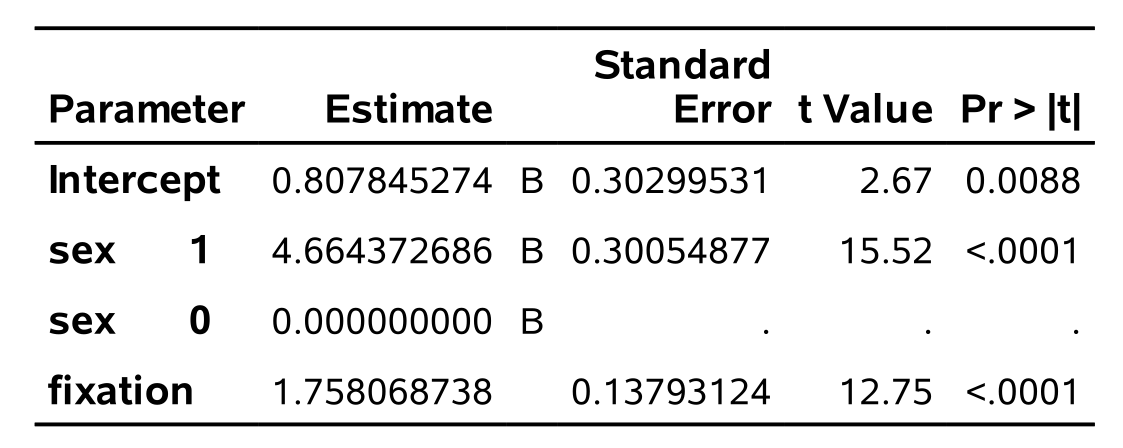
\includegraphics[width=0.65\linewidth]{img/c2/slides3-e18}
\end{figure}
{ \footnotesize All parameters are statistically significant at level $\alpha =0.05$.}
\end{frame}


 \begin{frame}[fragile]
  \frametitle{Illustration of interaction between continuous and binary variable}
  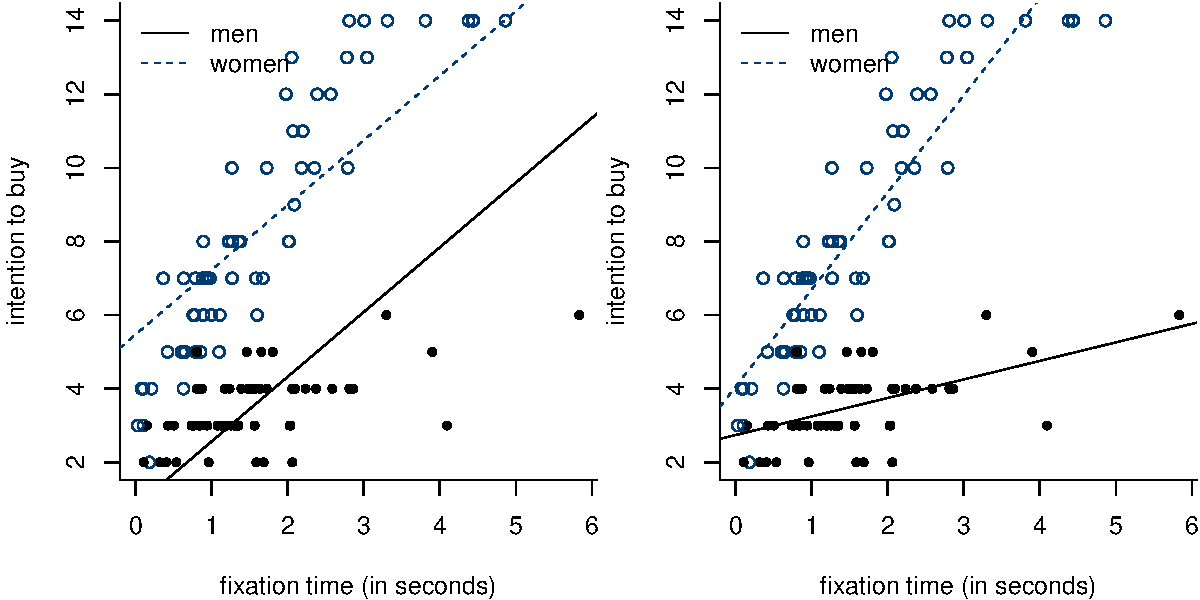
\includegraphics[width =\textwidth]{img/c2/03-linreg-interaction_cont.pdf}
 \end{frame}

\begin{frame}[fragile]
\frametitle{Modelling interactions}
\bi 
\item The previous figure shows that a better model would include a \alert{\textbf{different slope}} for men and women.
\item  In order to add a different slope for men and women, we can  \alert{create a new variable equal to the product} \code{fixation} $\cdot$ \code{sex}  and add it to the model,
{\small 
\begin{align*}
\code{intention} = \beta_0 + \beta_1 \code{sex} + \beta_2\code{fixation} + \beta_3 \code{fixation}\cdot \code{sex} + \varepsilon.
\end{align*} 
}
\item Depending on the value of the binary variable \code{sex}, we get
{\small 
\begin{align*}
\code{intention} = 
\begin{cases}
(\beta_0 + \beta_1) + (\beta_2 + \beta_3)\code{fixation} + \varepsilon, & \cif \code{sex}=1,\\
  \beta_0 + \beta_2 \code{fixation} + \varepsilon, & \cif \code{sex}=0.                  
\end{cases}
\end{align*} 
}
\item We recover the so-called \alert{main effect model}  when $\beta_3$ is zero. 
\ei
\end{frame}

 \begin{frame}[fragile]
\frametitle{Interaction between a continuous and a binary variable}
% \bi
% \item Here is the \SASlang code to fit the model with interaction
% \ei
\begin{tcolorbox}[colback=white,colframe=hecblue,title=\SASlang code to fit a linear model with an interaction]
{\small 
\begin{verbatim}
proc glm data=statmod.interaction;
class sex(ref="0");
model intention=sex fixation fixation*sex 
    / ss3 solution;
run;
\end{verbatim}
}
\end{tcolorbox}
\end{frame}
\begin{frame}
\frametitle{Parameter estimates of the interaction model}
\begin{center}
  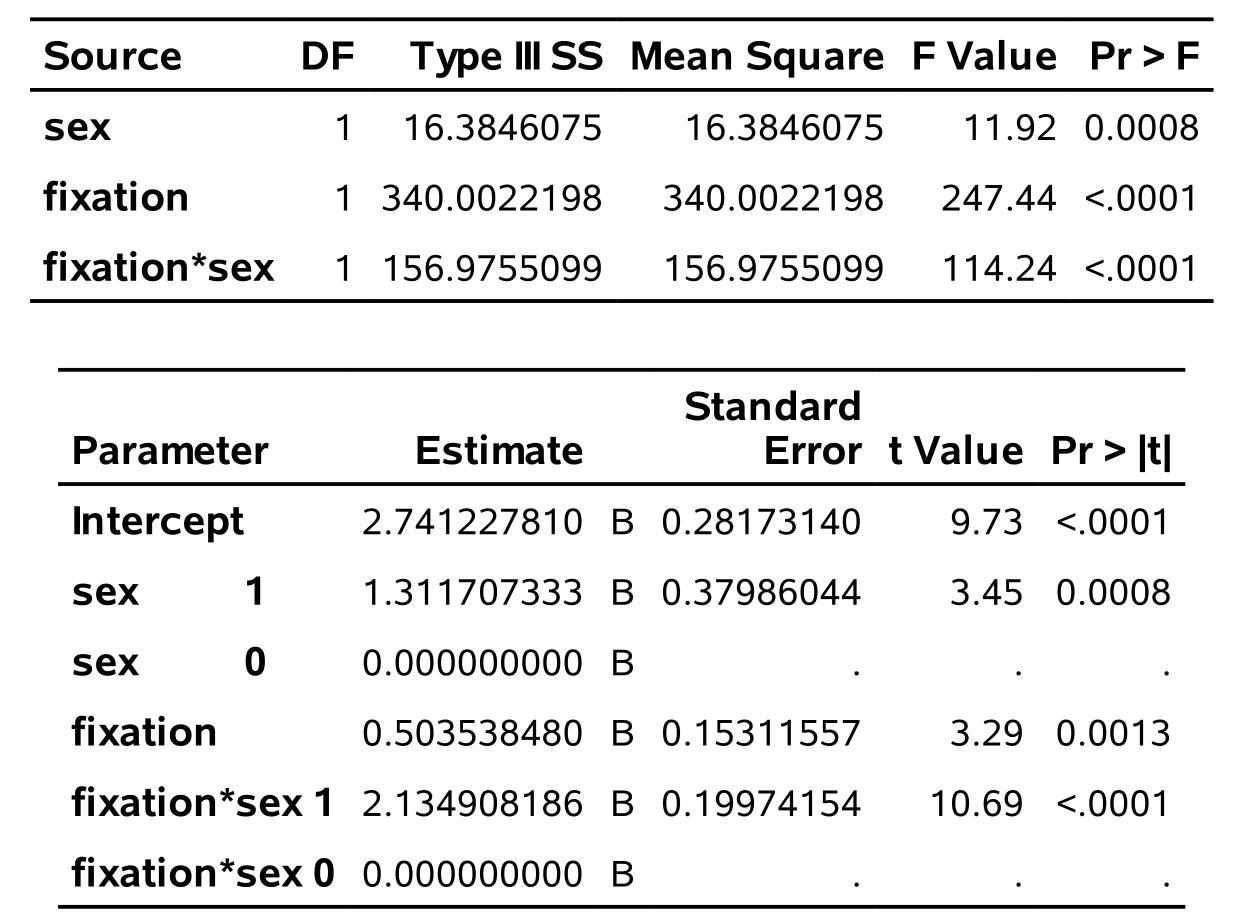
\includegraphics[width = 0.8\linewidth]{img/c2/slides3-e19}
\end{center}


 
% \item Once again, as we've seen for powers of a variable, it's possible to directly model the product of two variables using the command \code{model} for \code{proc glm}. 
% \bi
% \item \SASlang will consider \code{fixation}$*$\code{sex} as interaction term between the two covariates.
% \ei
\end{frame}

\begin{frame}
\frametitle{Interaction between a continuous and a binary variable}
\bi
% \item If we want to test whether the slopes are different, that is, if the effect of
% \code{fixation} is different according to the value of \code{sex}, \alert{we only need to test whether the parameter $\beta_3$ is significantly different from 0}. 
\item Testing whether the interaction is significant boils down to using the test $\Hy_0: \beta_3=0$.
\item If we reject $\Hy_0$, then there is a significant interaction between the two variables (in this case, the $p$-value is less than $0.0001$). 
\item The fitted model is
\bi
\item when \code{sex}$=0$, we have $\E{\code{intention}}=2.74+0.50  \code{fixation}$;
\item when \code{sex}$=1$, we have $\E{\code{intention}}=4.05+2.64  \code{fixation}$.
\ei
\item The concept of interactions readily extends to categorical variables with $k$ levels/categories.
\bi    
\item In this case, we need to use the global $F$-test to check if the interaction is statistically significant.
\ei
 \ei
\end{frame}


 \begin{frame}
\frametitle{Technical note}
\bi
\item The tests for \code{fixation} in the two tables are not the same because \code{fixation} is included in an interaction with a \code{class} variable. 
% The two $p$-values do not correspond to the same tests. 
\item In the table of coefficients, the $p$-value corresponds to the $t$-test for the two-sided hypothesis $\Hy_0:\beta_2=0$, i.e., the effect of \code{fixation} when \code{sex=0}. 
\item In the table above, the test is rather a test for the mean effect of \code{fixation},
\begin{align*}
\Hy_0: \{\beta_2+(\beta_2+\beta_3)\}/2=0
\end{align*}
\item These tests are \textbf{not} of interest. We cannot remove the main effect fixation unless we remove the interaction first. 
\ei
\end{frame}
\begin{frame}
  \frametitle{Main effects and arbitrary choice of baseline for factors}
  \bi \item In the model with buying \code{intention} as a fonction of \code{sex} and \code{fixation} time, we would \textbf{not} remove the main effect of \code{fixation} while keeping the interaction term \code{fixation*sexe}, even if we fail to reject $\Hy_0:\beta_2=0$.
  \item the parameter $\beta_2$ is the slope of \code{fixation} for men. Without it, the model would become
\begin{align*}
\code{intention} = 
\begin{cases}
(\beta_0 + \beta_1) + \beta_3\code{fixation} + \varepsilon, & \text{ if } \code{sex}=1,\\
  \beta_0 + \varepsilon, & \text{ if } \code{sex}=0;                 
\end{cases}
\end{align*}  
this implies that intention to buy is constant for me, regardless of the fixation time.
\item The choice of baseline is arbitrary, but changing the dummy \code{sex} (\code{0} for women, \code{1} for men), would yield a different model and so potentially different inferences.
\item The baseline would not anymore be arbitrary!
\ei
 \end{frame}
 
 
\begin{frame}
\frametitle{Interactions between categorical variables}
\bi
\item For two categorical variables with respectively $k_1$ and $k_2$ levels, the interaction model has \[k_1k_2 = 1+ (k_1-1) + (k_2-1) + (k_1-1)(k_2-1)\] parameters --- one for each combination.
\item The number of restrictions to go from interaction model to main effect model is thus $(k_1-1)(k_2-1)$.
\item The interpretation of the main effects are as before, i.e., they represent contrasts relative to a baseline, but the latter is level-dependent.
\item We consider interaction terms \textbf{only if} the corresponding main effects are included.
\item If the variance of the subgroup are equal, we can test the restriction using the $F$-statistic for global effects.
\ei
\end{frame}

\begin{frame}[fragile]
 \frametitle{Interactions between categorical variables}
  \bi 
 \item Consider a model for residual health insurance charges as a function of smoking and obesity indicators, after accounting for the effect of age.
 \item The fitted average for each group is based on the model
\begin{align*}
\code{rcharges} = \beta_0 + \beta_1 \code{smoker} + \beta_2 \code{obese}_1 +  \beta_3 \code{obese}_2 + \eps. 
\end{align*}
where $\code{obese}_1=1$ if $25\leq \code{bmi} < 30$ (overweight) and $\code{obese}_2=1$ if $\code{bmi} \geq 30$ (obese).
\ei

\end{frame}
\begin{frame}[fragile]
 \frametitle{Graphical representation of interactions between categorical variables}
\begin{figure}
 \centering
 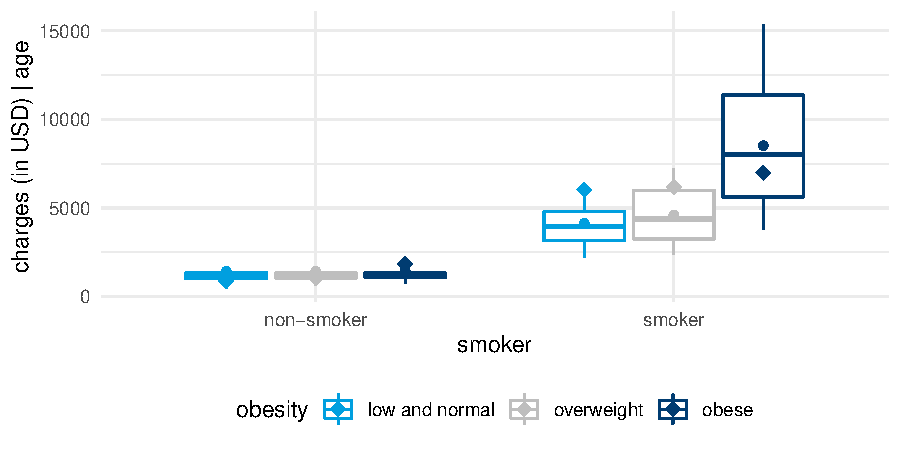
\includegraphics[width = 0.8\linewidth]{img/c2/03-linreg-interaction_categ.pdf}
\end{figure} 
{\tiny 
The diamonds indicate the fitted value for each group for the main effect, whereas the dots show the fitted values for the interaction model (mean of each group). The health insurance charges are clearly higher for obese smokers, something the main effect model fails to capture: it underpredicts the charges of obese smokers and overpredicts that of non-obese smokers.  \par
}
\end{frame}
\begin{frame}[fragile]
\frametitle{Interaction model with two categorical variables}
The linear model with interaction is
{ \small 
\begin{align*}
\code{rcharges} &= \beta_0 + \beta_1 \code{smoker} + \beta_2 \code{obese}_1 +  \beta_3 \code{obese}_2 \\ & \quad \beta_4\code{smoker}\cdot\code{obese}_1  + \beta_5\code{smoker}\cdot\code{obese}_2  + \eps. 
\end{align*}
}
The average charge for 
{\small 
\bi 
\item non-smokers with body mass index less than 25 is $\beta_0$;
\item overweight non-smokers is $\beta_0 + \beta_2$;
\item obese non-smokers is $\beta_0 + \beta_3$;
\item obese smokers is $\beta_0 +\beta_1+  \beta_3 + \beta_5$\ldots 
\ei
}
Testing for the interaction amounts to $\Hy_0: \beta_4=\beta_5=0$.
\end{frame}
\begin{frame}[fragile]
\frametitle{Interpretation of parameters in the interaction model}
The linear model with interaction is
{ \small 
\begin{align*}
\code{rcharges} &= \beta_0 + \beta_1 \code{smoker} + \beta_2 \code{obese}_1 +  \beta_3 \code{obese}_2 \\ & \quad \beta_4\code{smoker}\cdot\code{obese}_1  + \beta_5\code{smoker}\cdot\code{obese}_2  + \eps. 
\end{align*}
}
 \bi
  \item The interpretation is as before (but less straightforward\ldots)
{\footnotesize  
\bi
\item $\beta_0$, the baseline, is the mean charges of people whose body mass index (BMI) is less than 25 who do not smoke.
\item $\beta_1$ is the difference between the mean charges of smokers and non-smokers for individuals whose BMI is less than 25.
\item $\beta_2$ is the difference between the mean charges  for overweight non-smokers and non-smokers whose BMI is less than 25.
\item $\beta_3$ is the difference between the mean charges  of obese non-smokers and that of non-smokers whose BMI is less than 25.
\item $\beta_2 + \beta_4$ is the difference between the mean charges  for overweight smokers and smokers whose BMI is less than 25.
\item $\beta_3 + \beta_5$ is the difference between the mean charges  of obese smokers and that of smokers whose BMI less than 25.
\ei
}
\ei
\end{frame}



\begin{frame}
\frametitle{Higher-order interaction}
\bi
% \item  The preceding examples showed second-order interactions; that is, interaction between two variables. 
\item In theory, we could consider an \alert{interaction between any number of variables}. However, in practice we rarely go higher than third-order because it quickly becomes difficult to interpret the effects. Additionally, estimating an interaction between several variables requires a very large sample size. 
\item The basic principle is still the same. To create an interaction of a given order between several variables, we also need to include all the lower-order terms between the variables included in the higher-order interaction term. 
\item We interpret the variable effects while fixing the values of all the other variables in the interaction term. 
\ei
\end{frame}

\begin{frame}[fragile]
\frametitle{Final remarks on interactions}
\bi
% \item It's usually preferable to include all possible interactions of order less than the maximum order interaction included in the model. 
\item Don't remove a lower-order term, even if it's not significant.  The lower-order terms are needed for proper inference!
\item While it is tempting to include interactions between many categorical variables, beware of sparsely populated sub-categories.
\item Algorithms performing model selection often base their variable choice on  predictive performance.
\bi \item removing lower-order term may not matter for the development of a black-box predictive model.
\ei 
\item However, removing main effects implies that the baseline is \textbf{not arbitrary} and inference is \textbf{invalid}.
% \item One exception is when we're developing a predictive model and we don't plan on testing individual variables.  We would then include all the variables, as well as several (or even all) interaction terms and let an algorithm choose the best model. 
% \item This algorithm will not necessarily respect the above rule, but this won't matter as we only care about predictive performance.
\ei
\end{frame}
\end{document}
